\documentclass[11pt,a4paper]{article}

\usepackage[a4paper,top=2cm,bottom=2cm,left=3cm,right=3cm,marginparwidth=1.75cm]{geometry}
\usepackage{graphicx}
\usepackage{amsmath}
\usepackage{booktabs}
\usepackage{float}
\usepackage{setspace}
\usepackage{titlesec}
\usepackage{parskip}

\usepackage[colorlinks=true,       % Enlaces en color, NO en recuadro
            linkcolor=black,       % Color de enlaces internos
            urlcolor=blue,         % Color de URLs
            citecolor=black,       % Color de citas
            pdftitle={Predicting the FIFA World Cup 2026},
            pdfauthor={Javier Ruano Hernández},
            pdfsubject={Monte Carlo Simulation},
            pdfkeywords={football, prediction, monte carlo, world cup},
            pdfborder={0 0 0},     % ¡ESTO QUITA EL RECUADRO!
            breaklinks=true,       % Permite que los URLs largos se rompan
            hyperfootnotes=false]{hyperref}

% Para abrir enlaces externos en nueva pestaña
\usepackage{hyperref}
\hypersetup{
    linktocpage,  % Enlaces de TOC a páginas, no secciones
    pdfnewwindow=true  % ¡Esto hace que los enlaces externos se abran en nueva pestaña!
}

\setstretch{1.15}

\titleformat{\section}{\Large\bfseries}{\thesection.}{0.5em}{}
\titleformat{\subsection}{\large\bfseries}{\thesubsection.}{0.5em}{}

\title{\textbf{Predicting the FIFA World Cup 2026}\\
\large A Monte Carlo Simulation of Modern Tournament Football}

\author{
    \textbf{Javier Ruano Hernández} \\
    \small
    \href{https://github.com/javierruanohdez/}
    {\color{githubblue}\textbf{javierruanohdez}}
}
\date{\today}


\begin{document}
\maketitle

\begin{center}
    
\includegraphics[width=0.9\textwidth]{assets/cover_image.jpg}
\end{center}

\begin{abstract}
Predicting the outcome of a football World Cup is inherently uncertain. Traditional odds and statistical models often fail to capture the complex interplay of modern football dynamics, including tactical evolution, squad rotation, momentum, and tournament-specific randomness. 

\bigskip

This work presents a Monte Carlo simulation framework for the FIFA World Cup 2026, integrating historical team performance, FIFA rankings, recent form, head-to-head statistics, and a modern football strength metric.

\bigskip

By running thousands of tournament simulations, the model generates probabilistic estimates for championship outcomes, highlighting both favorites and potential dark horses. Our approach emphasizes structural and tactical consistency over mere historical prestige, providing a complementary perspective to conventional betting markets. Notably, the final showdown between Spain and Argentina emerges as a particularly revealing scenario, pitting two of the most robust and tactically adaptive teams against each other under conditions of extreme variance.

\end{abstract}

\clearpage

\section{Introduction}

Football resists precise prediction. Unlike league competitions, World Cups are short, intense, and unforgiving. A single draw, red card, or penalty shootout can overturn years of planning.

Traditional approaches rely heavily on historical prestige or betting odds. However, recent tournaments have shown that:
\begin{itemize}
    \item Tactical cohesion often outweighs individual talent
    \item Teams peak at different moments
    \item Variance increases dramatically in knockout stages
\end{itemize}

The 2026 World Cup introduces an expanded format and three host countries, further increasing uncertainty. This project aims to model that uncertainty explicitly.

\section{World Cup 2026: Structural Challenges}

The 2026 FIFA World Cup differs fundamentally from previous editions:
\begin{itemize}
    \item Hosted across the United States, Canada, and Mexico
    \item Long travel distances between venues
    \item Climate and time-zone variability
    \item Expanded format with 48 teams
\end{itemize}

The tournament structure consists of:
\begin{itemize}
    \item 12 groups of 4 teams
    \item 12 group winners qualify automatically
    \item Best 8 runners-up advance
    \item Remaining runners-up play a preliminary knockout round
    \item Standard knockout stages from Round of 16 onward
\end{itemize}

This structure increases exposure to randomness, particularly for traditional powerhouses that historically rely on slow tournament starts.

\clearpage

\section{Data Sources}

The model integrates multiple data sources:

\subsection{Match Results}

Historical international match results from 2000 onward were derived from a publicly available dataset hosted on Kaggle, originally compiled by Mart Jürisoo. The dataset aggregates official international matches dating back to 1872 and is widely used in football analytics research.

\subsection{FIFA Rankings}

FIFA ranking points were collected across multiple years. While FIFA rankings are imperfect, they provide a standardized proxy for baseline team strength and seeding expectations.

\subsection{Tournament Achievements}

A custom dataset of tournament achievements was constructed with the assistance of AI-based data structuring. This dataset encodes:
\begin{itemize}
    \item World Cup titles, finals, and semifinal appearances
    \item Continental titles, finals, and semifinal appearances
    \item Recency of achievements with exponential decay
\end{itemize}

The goal is to reward recent competitive relevance rather than distant history.

\section{Methodology}

\subsection{Match-Level Model}

Individual matches are evaluated using a Gradient Boosting classifier trained on:
\begin{itemize}
    \item FIFA point differentials
    \item Recent form (smoothed last five matches)
    \item Head-to-head statistics
    \item Interaction features between form and ranking
\end{itemize}

Predicted probabilities are adjusted to reflect tournament round variance.

\subsection{Tournament Simulation}

Each World Cup simulation represents one plausible tournament universe. For each simulation:
\begin{enumerate}
    \item Group stages are played match by match
    \item Qualification follows official 2026 rules
    \item Knockout rounds introduce increasing randomness
\end{enumerate}

A total of 5,000 simulations were executed to obtain stable probability estimates.

\subsection{Variance by Tournament Round}

Randomness increases as the tournament progresses:

\begin{verbatim}
Group stage      → Low variance
Round of 16      → Medium variance
Quarterfinals    → High variance
Final            → Maximum variance
\end{verbatim}

This reflects empirical tournament behavior.

\section{Modern Football Strength}

A key modeling decision is the inclusion of a ``modern football strength'' component.

Historical success alone does not guarantee present competitiveness. This component rewards:
\begin{itemize}
    \item Tactical continuity
    \item Pressing systems and compact blocks
    \item Squad automation and positional discipline
    \item Post-2018 tournament performance
\end{itemize}

Teams such as Argentina, Spain, France, England, and Morocco score highly under this framework.

\section{Results}

After 5,000 simulations, the estimated probabilities of winning the tournament are summarized below:

\begin{center}
\begin{tabular}{lr}
\toprule
Team & Probability (\%) \\
\midrule
Argentina & 16.1 \\
Spain & 13.1 \\
France & 12.8 \\
Portugal & 8.5 \\
England & 8.4 \\
Croatia & 5.2 \\
Germany & 4.9 \\
Morocco & 4.7 \\
Belgium & 4.1 \\
Brazil & 2.9 \\
\bottomrule
\end{tabular}
\end{center}

While betting markets often favor Spain marginally, the simulation consistently places Argentina at the top due to stability, adaptability, and recent tournament performance.

\vspace{1em}

\begin{figure}[H]
\centering
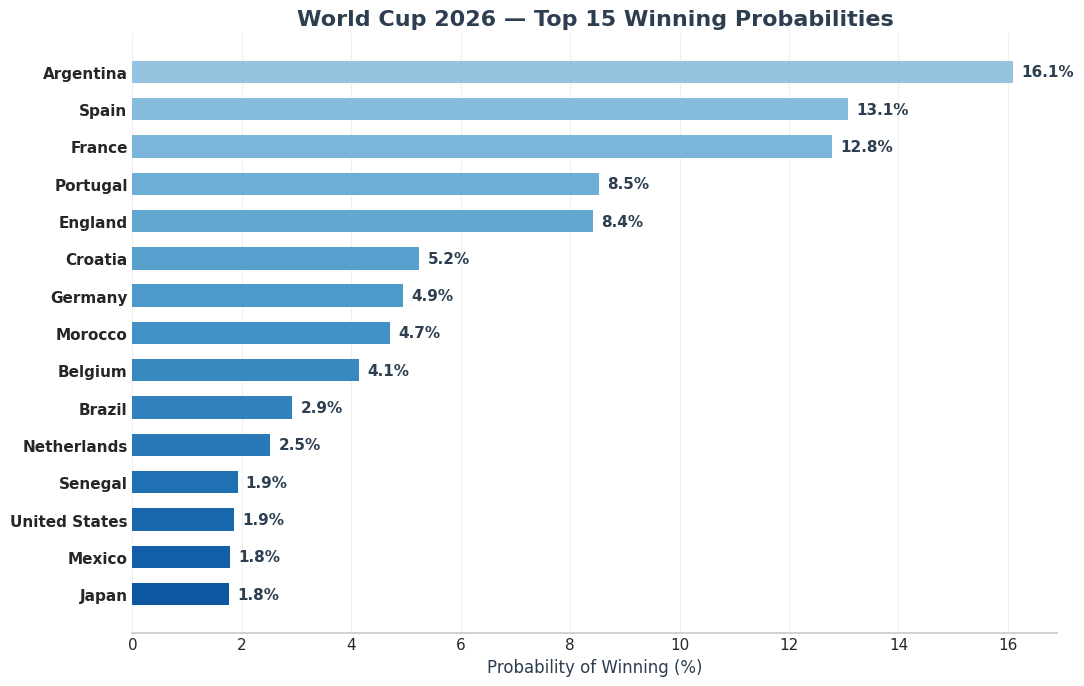
\includegraphics[width=0.9\textwidth]{simulation_results/top15_probabilities.png}
\caption{Top 15 team probabilities of winning the World Cup 2026.}
\end{figure}

\begin{figure}[H]
\centering
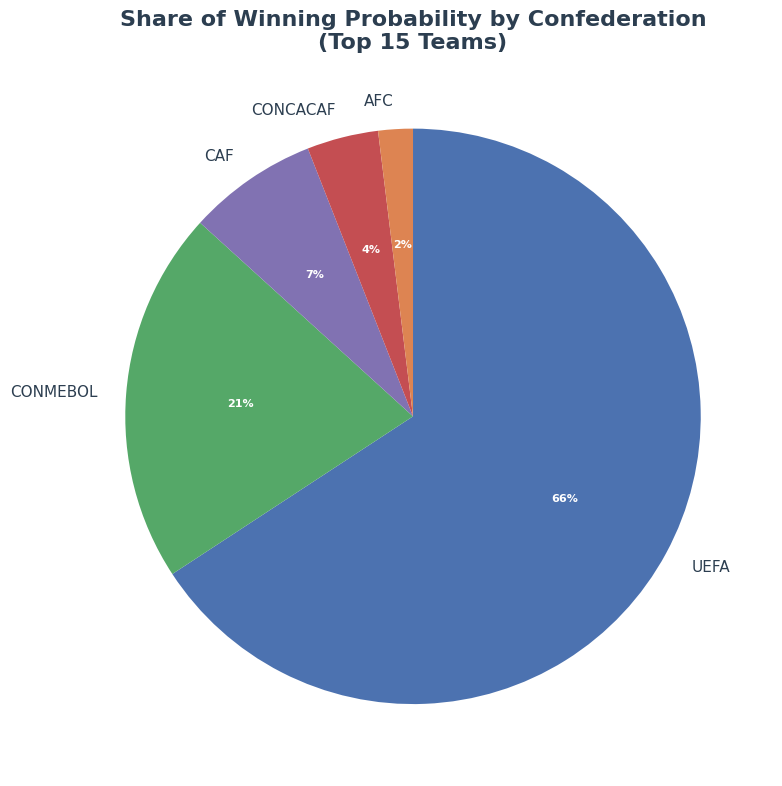
\includegraphics[width=0.7\textwidth]{simulation_results/confederation_share.png}
\caption{Distribution of winning probabilities by confederation (Top 15 teams).}
\end{figure}

\begin{figure}[H]
\centering
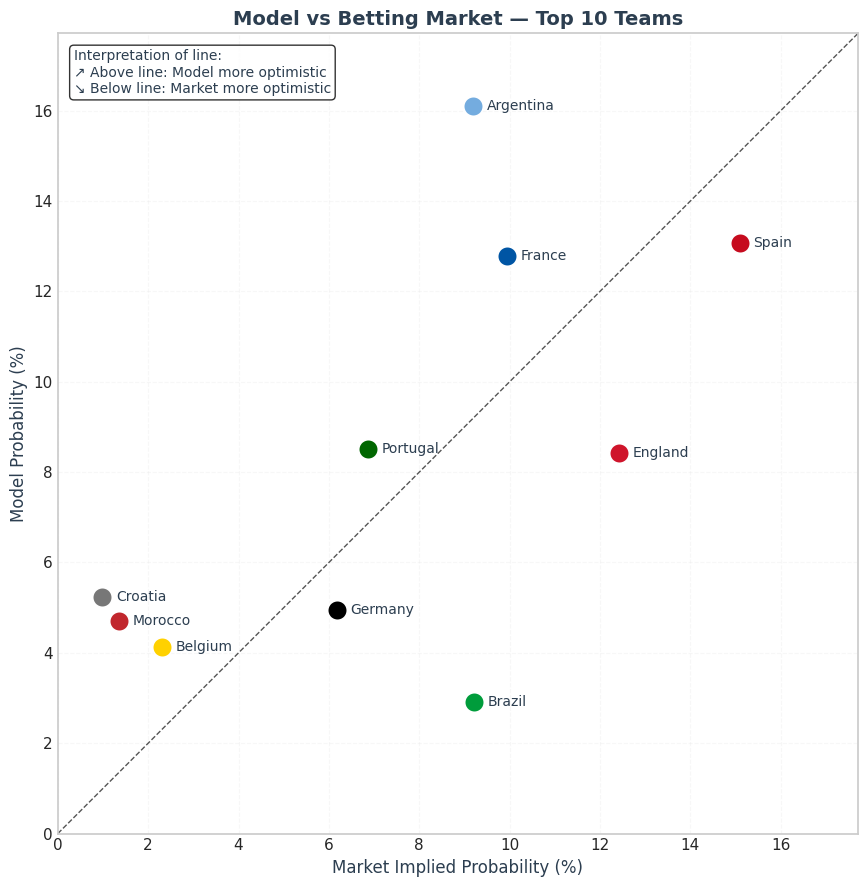
\includegraphics[width=0.8\textwidth]{simulation_results/model_vs_market_top10.png}
\caption{Comparison between model predictions and market implied probabilities (Top 10 teams).}
\end{figure}

\section{Interpretation}

The model answers a different question than bookmakers:
\begin{quote}
Which teams are best adapted to modern tournament football under extreme variance?
\end{quote}

Under this lens:
\begin{itemize}
    \item Argentina exhibits the highest consistency
    \item Spain and France form a closely matched second tier
    \item Portugal and England benefit from tactical maturity
    \item Croatia and Morocco emerges as dark horses due to structure and resilience
\end{itemize}

The upcoming Finalissima between Spain and Argentina is particularly revealing, as it pits the two most consistently favored teams in the simulation against each other in a competitive setting.

\clearpage

\section{Limitations}

This model has important limitations:
\begin{itemize}
    \item No explicit modeling of injuries or squad selection
    \item Coaching changes are not dynamically updated
    \item Player-level form is aggregated at team level
    \item FIFA rankings introduce structural bias
\end{itemize}

Most importantly, football remains inherently unpredictable.

\section{Future Work}

Potential extensions include:
\begin{itemize}
    \item Player-level embeddings based on club performance
    \item Travel and climate fatigue modeling
    \item Tactical matchup vectors
    \item Real-time odds comparison
\end{itemize}

\section{Conclusion}

This project does not aim to predict the World Cup with certainty. Instead, it embraces uncertainty and uses it as a modeling feature.

The Monte Carlo approach allows us to see not just a winner, but the distribution of possible outcomes, highlighting which teams are structurally robust under variance.

Graphical results demonstrate that:
\begin{itemize}
    \item Argentina consistently ranks highest across simulations
    \item Spain and France remain highly competitive, often neck-and-neck
    \item England, Portugal, Croatia, Germany and Morocco show variability that could make knockout surprises likely
    \item Confederation distribution highlights the relative strength of UEFA and CONMEBOL teams in the top tier
    \item Market comparison plots reveal where betting odds diverge from model insights
\end{itemize}

In summary, modern football prediction benefits from combining historical data, tactical evaluation, and simulation under uncertainty. While no model can fully capture the chaos of a tournament, this approach provides both insightful probabilities and a framework for strategic understanding.

\end{document}